\section{Mean Shift}

The principle of the Mean shift is to move a window over the data set following the density gradient. This method take the bandwidth for the window as parameter.\\
\begin{figure}[h!]
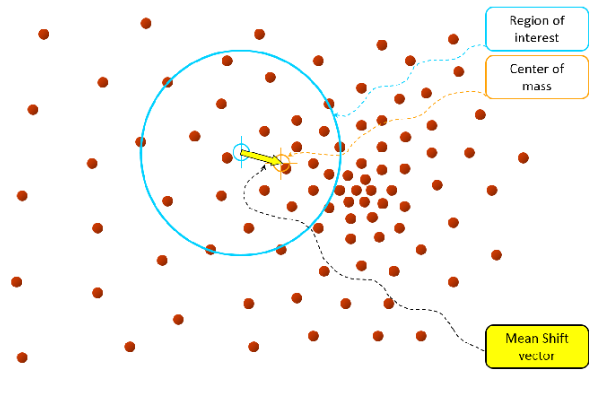
\includegraphics[width=0.3\textwidth, height=5.5cm]{Image/algo-meanshift1.png}
\end{figure}

We first take a random point. Each point in this window will be in this cluster. We compute the mean of these points.




\begin{figure}[h!]
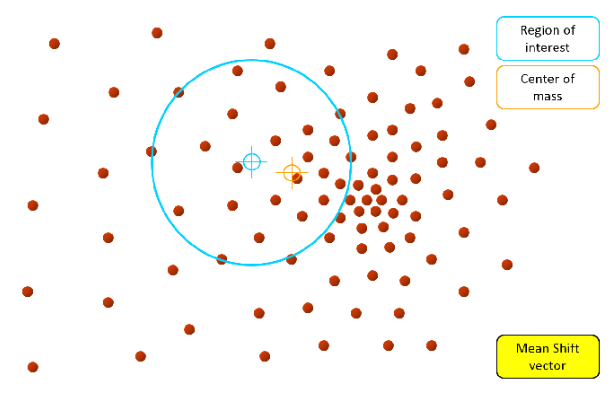
\includegraphics[width=0.3\textwidth, height=5.5cm]{Image/algo-meanshift2.png}
\end{figure}



\begin{figure}[h!]
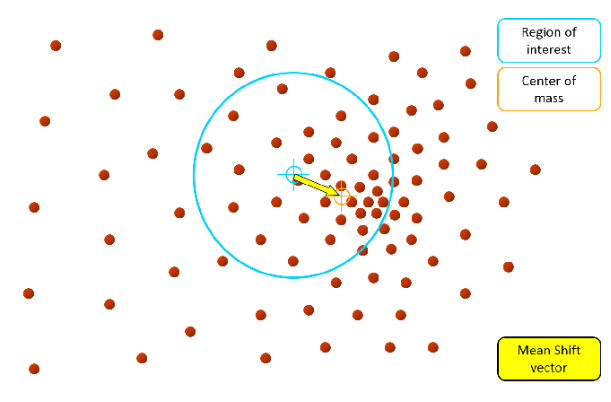
\includegraphics[width=0.3\textwidth, height=5.5cm]{Image/algo-meanshift3.png}
\end{figure}


This mean becomes the new window center, and we move the window following the density gradient until the difference between the center and the mean gets close to 0.


Then we apply this again for a point that does not belong to any cluster, until every point is affected to a cluster. The algorithm can also merge the closest clusters, depending on the bandwidth.
The main benefit of this method is that it does not need to get the number of clusters as parameter.

